\section{Analysis}
\subsection{Performance}
Fahri et al. demonstrated the performance of QAOA on several types of graphs \cite{farhiQAOA}. A 2-regular graph is a graph in which each vertex has two edges and contains one or more (disconnected) cycles \cite{farhiQAOA}. For a 2-regular graph, QAOA is able to provide an approximation ratio: $\alpha \geq (2p + 1)/(2p + 2)$ \cite{farhiQAOA}. This is significant because this approximation ratio does not depend on the problem size, only on p (number of layers). Moreover, the approximation ratio increases with increasing p, which means that with high enough p, QAOA can find a solution close to the optimal. More approximation ratios for QAOA are shown in the table (see Table 1) \cite{farhiQAOA, 2018Wurtz_2021, 19HALPERIN2004169}. 

\begin{table}[H]
\centering
\resizebox{8cm}{!}{ % Resize table to fit the text width
\begin{tabular}{||c c c c||} 
 \hline
 Graph Type & Algorithm & Parameters & Approx. Ratio \\ [0.4ex] 
 \hline\hline
 2-regular & QAOA & for any p & $\alpha \geq \frac{(2p+1)}{(2p+2)}$ \\ 
 \hline
 3-regular & QAOA & p = 1 & $\alpha \geq 0.6924$ \\
 \hline
 3-regular & QAOA & p = 2 & $\alpha \geq 0.7559$ \\
 \hline
 3-regular & QAOA & p = 3 & $\alpha \geq 0.7924$ \\
 \hline
 Any graph & GW & N/A &  $\alpha \geq 0.8786$\\ 
 \hline
 $\leq$ 3-regular & SDP & N/A & $\alpha \geq 0.9326$ \\[1ex] 
 \hline
\end{tabular}
}
\caption{Approximation ratios for QAOA and classical algorithms for different graph types. From \cite{farhiQAOA, 2018Wurtz_2021, 19HALPERIN2004169}}
\label{table:1}
\end{table}

\subsection{Classical Algorithms}
The proven lower bounds for QAOA are lower than the existing best-known classical algorithms, such as the Goemans-Williamson algorithm. However, the benefit of QAOA comes with its increasing approximation ratio with increasing layers, p, and the fact that this does not depend on the system size. It is difficult to theoretically prove a lower bound for high p due to the increasing complexity, so classical algorithms still give higher theoretical worst-case bounds for approximation ratios.

\subsubsection{Goemans-Williamson Algorithm}
The Goemans and Williamson (GW) algorithm is the best approximation algorithm for MaxCut problems. They found a 0.87856 approximation ratio, an improvement over the previous best of 0.5 by Sahni and Gonzales \cite{GWalgorithm, 204569755}. This algorithm is considered a semidefinite program, a type of problem concerned with optimizing a linear cost function with the requirement that the matrix is positive semidefinite \cite{GWalgorithm}.

The idea behind the algorithm is to relax the constraint that each vertex can only be two values and instead let it be any vector with a magnitude of 1 \cite{GWalgorithm}. When applying the dot product: $x_i \centerdot x_j$, we have a positive semidefinite matrix. Out of the possible solution vectors $x_i$, choose a random hyperplane through the origin and assign all those vectors that lay above to be part of one partition, and all those below to the other. This procedure is often known as "rounding" in semidefinite programming. Given this approximation ratio of 0.87856, we can see that the ratios from QAOA do not beat this, but there is still a lot to be studied and tested at larger system sizes and QAOA layers. 

The classical algorithm can compute an approximation in polynomial time, which requires significant computational resources for large graphs \cite{GWalgorithm}. In contrast, the computational complexity for QAOA increases with the number of layers, p. The point where QAOA could surpass the classical algorithms depends on the graph structure, number of layers (p) and hardware capabilities.

\subsection{Comparison to Classic Quantum Algorithms}
Recall how phase kickback is a cornerstone to many classic quantum algorithms such as Grover's and Shor's. Phase estimation uses phase kickback to extract the phase of the eigenvalue \cite{classBook}. The number of qubits we use in this algorithm is the number of decimal places of precision we achieve for the phase. This is similar to QAOA in that with a higher circuit depth (larger number of layers), the accuracy of the approximation improves. However, this also means that in order to achieve high precision in phase estimation, a large number of qubits is required, causing phase estimation to be less suitable on NISQ devices than algorithms like QAOA. QAOA's dependence on the number of layers for accuracy, rather than the number of qubits, combined with its hybrid quantum-classical framework, makes it a strong candidate for execution on NISQ devices.

Grover's is another classic quantum algorithm that provides quadratic speedups for unstructured search problems \cite{classBook}. Grover's algorithm is able to provide exact solutions, unlike QAOA's approximate solutions. However, Grover's still requires a lot of qubits and minimal errors. Therefore, it will most likely not see practical use until fault-tolerant quantum computers exist. Grover's algorithm and QAOA share a similarity in their iterative approaches within quantum circuits: Grover's algorithm repeatedly applies the Grover operator to amplify the probability of the desired outcome, while QAOA executes multiple layers of its parameterized quantum circuit to optimize the solution.

While these algorithms all have different purposes and applications, they share some similarities in how the circuits are created and in their performance. QAOA acts more as an intermediate algorithm between classical optimization and the long-term potential of fully fault-tolerant algorithms such as Grover's, Shor's, and phase estimation.

\subsection{Results}
\subsubsection{Simulated Results}
In 2018, Crooks at Rigetti simulated the performance of QAOA on MaxCut with a variety of layers and graph sizes \cite{24crooks2018performancequantumapproximateoptimization}. He found that at $p \geq 8$, the performance of QAOA exceeds that of the Goemans-Williamson algorithm \cite{24crooks2018performancequantumapproximateoptimization} (see Fig 4).

\begin{figure}[H]
    \centering
    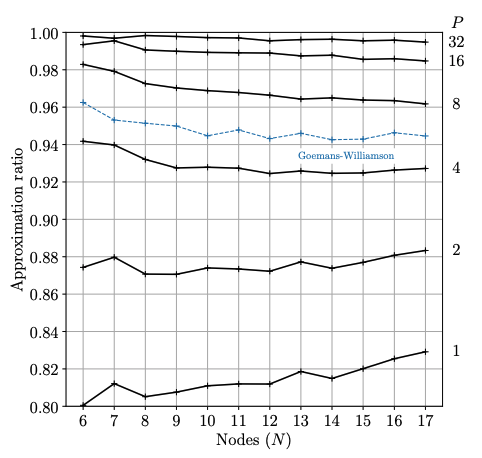
\includegraphics[width=1\linewidth]{images/CrooksResults.png}
    \caption{Results from Crooks \cite{24crooks2018performancequantumapproximateoptimization} Approximation ratio of QAOA on MaxCut with various graph sizes (N) and QAOA layers (P). The blue line demonstrates the performance of the Goemans-Williamson algorithm.}
    \label{fig:4}
\end{figure}

Lotshaw et al. later simulated the performance of QAOA on all connected non-isomorphic graphs for $n \leq 9$ vertices \cite{26Lotshaw_2021}. The simulation was done for QAOA layers p = 0, 1, 2, and 3 (see Fig 5). We can see that for p = 2 and 3, QAOA performs better than GW up to 9 vertices. Interestingly, in these experiments, the performance of QAOA seems to converge to a value, suggesting that the performance may stabilize as system size increases.

\begin{figure*}
    \centering
    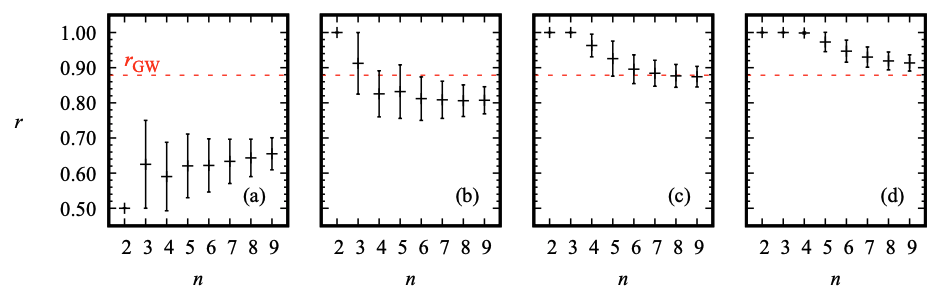
\includegraphics[width=1\linewidth]{images/lotshawResults.png}
    \caption{Results from Lotshaw \cite{26Lotshaw_2021} where n is the number of vertices and r is the approximation ratio. The four panels show p = 0, 1, 2, 3 from left to right. The red dashed line shows the approximation ratio of the Goemans-Williamson algorithm.}
    \label{fig:enter-label}
\end{figure*}

While no proven theoretical bounds better than classical have been established, QAOA shows immense promise for higher p and larger systems.

\subsubsection{Results on Real Quantum Hardware}
Running QAOA on real quantum computers introduces many extra factors, including decoherence and noise. While theoretically, as p increases, the approximation ratio should continue increasing for QAOA, this is certainly not the case when we have to consider noise and errors.

A team demonstrated the performance of QAOA on the Google Sycamore superconducting processor in 2021 \cite{27harrigan2020nonplanargraphs}. They ran simulations and experiments on three types of problems: MaxCut on 3-Regular graphs, Hardware grid, and Sherrington-Kirkpatrick (SK) Model. The authors found that performance increased up until p = 3, after which the noise that comes with larger circuit depth outweighed the improvement by increasing p \cite{27harrigan2020nonplanargraphs}.

Bengtsson et al. also performed experiments to test the performance of QAOA on small quantum processors \cite{28bengtsoon2019improved}. The authors found that for p = 2 with covariance matrix adaptation evolution strategy for the classical optimization part, the success probability was 96.6\% \cite{28bengtsoon2019improved}. However, they noticed that the success probability decreased for p = 3 (94.2\%) due to increased gate count \cite{28bengtsoon2019improved}.

An interesting comparison of the performance of QAOA is quantum annealing (QA). The QAOA can be thought of as a form of quantum annealing using discrete time steps and shrinking the time steps to become extremely small ($p \rightarrow \inf$) \cite{25Willsch_2020}. The author tested MaxCut on an IBM simulator, IBM Q 16 Melbourne processor, and D-Wave \cite{25Willsch_2020}. The performance of the IBM Q processor was very bad compared to the simulator, suggesting that noise has a significant impact \cite{25Willsch_2020}. For a problem with 18 vertices, the D-wave machine demonstrated an approximation ratio of 0.91, while QAOA simulated with p = 5 resulted in a ratio of 0.87 \cite{25Willsch_2020}.

\subsection{Variations}
Several improvements have been made to QAOA that are worth noting. These include warm-starting QAOA, conditional value at risk, optimizing the circuit, testing other ansatzes and many more.

\subsubsection{Warm Starting}
The idea behind warm starting quantum optimization (WS-QAOA) is to use classical algorithms to provide the initial state to QAOA, giving it a "headstart" \cite{29egger2020warmstarting}. Any classical algorithm, such as the semidefinite programming techniques in 4.2, can be used to initialize the quantum algorithm. In order to do this, the mixer Hamiltonian needs to be changed to one with the given initial state as ground state \cite{29egger2020warmstarting}. A further variation is to include GW rounding to further optimize the initial state to ensure that WS-QAOA is at least as good as GW \cite{29egger2020warmstarting}. The idea of WS-QAOA is that if we give it an initial state closer to the optimal, it will converge faster than regular QAOA and will, therefore, require lower p.

The authors found that in a simulation, the probability of finding the optimal solution was 5 times higher for WS-QAOA than with standard QAOA for depths $1 \leq p \leq 5$ \cite{29egger2020warmstarting}. They also found that the quality of the solution that the WS-QAOA found was better than standard QAOA.

\subsubsection{Recursive QAOA}
Bravyi et al. in 2019 propose a non-local version of QAOA, recursive QAOA (RQAOA), addressing some of the limitations caused by the locality and symmetry of QAOA \cite{31bravyi2018obstacles}. RQAOA uses QAOA to identify strong correlations between the variables in the problem at hand \cite{31bravyi2018obstacles}. Standard QAOA is first run; then one variable is fixed based on the outcome, which reduces the problem size. This is repeated recursively until the problem is small enough to be solved classically. The authors ran a numerical comparison with p = 1 on system sizes n = 32 and n = 100 to compute the approximation ratios for different problems for standard QAOA and RQAOA \cite{31bravyi2018obstacles}. They found that RQAOA performed significantly better than standard QAOA. Researchers have also applied warm starting to RQAOA (WS-RQAOA), getting even better results than WS-QAOA, RQAOA, and QAOA \cite{29egger2020warmstarting}.

\subsubsection{CVaR (Conditional Value-at-Risk)}
Another improvement to QAOA was made by Barkoutsos et al. in 2020, in which the authors propose that instead of minimizing the expectation value, minimize the CVaR \cite{30barkoutsos2020}. CVaR is a measure that only takes a fraction of the outcomes, considering only the tail end of the probability distribution \cite{30barkoutsos2020}. The researchers found that this change allowed the algorithm to find the solution quicker in both simulations and on real quantum hardware \cite{30barkoutsos2020}.

\subsection{Limitations}
Theoretically, the approximation ratio should increase for QAOA as the number of layers (p) increases. However, this improvement is not always realized due to the noisy and error-prone nature of current quantum hardware. The performance of QAOA can be further affected by increased graph sizes, which require more qubits, amplifying the impact of hardware limitations like decoherence and gate errors. Moreover, optimizing the variational parameters poses a significant challenge; the classical optimization step becomes computationally expensive as the number of parameters grows with larger p. Even though the QAOA is thought to be an algorithm for noisy computers, the current devices still do not match the requirements for the algorithm to outmatch its classical counterparts. Its performance can heavily depend on the structure of the problem. 

Sanders et al. optimized circuits of various quantum optimization algorithms, including QAOA, to test if they would be able to be run on a small fault-tolerant quantum computer \cite{Sanders_2020}. They found that despite optimizing the compiled quantum circuits as much as possible, hundreds of thousands of qubits would be necessary to be able to run a problem of size n = 64 with error rates on the order of $10^{-4}$. This highlights some of the hardware requirements needed to effectively run QAOA on larger problems.